%% CAPITOLO 3
\clearpage
\chapter{Progettazione dell'architettura}\label{ch:design}
In questo capitolo vengono descritti i sistemi realizzati dal punto di vista architetturale.
Innanzitutto, verrà descritto l'ETL realizzato per il calcolo dei rendimenti e come è stata iniziata l'integrazione del nuovo PFP all'interno del progetto.
Poi, verrà analizzata la componente realizzata per il prodotto di Baseline, spiegando quanto è stato fatto durante il tirocinio e quanto è stato progettato per i periodi successivi.
Infine, verrà descritta l'infrastruttura e le tecnologie utilizzate per l'hosting di risorse e programmi.

\section{ETL dei rendimenti e PFP}\label{sec:etl-architecture}
Al momento dell'inizio del tirocinio curriculare, il progetto era già stato iniziato.
Di conseguenza, il lavoro svolto si limita all'implementazione del progetto già pianificato.
In questa sezione viene descritta l'architettura del sistema realizzato specificando quali cambiamenti vi sono stati rispetto alla fase di progettazione.

Come descritto nell'introduzione alla problematica (sezione~\ref{subsec:problem-analysis}), l'integrazione di dati è un processo molto complesso ed estremamente personalizzato;
in questo senso, non vi è uno \textit{standard de facto} da seguire per progettare l'\textit{ETL} aziendale, tuttavia esiste una sorta di percorso che indica il modo in cui sia da effettuare l'integrazione.
Tale percorso considera i seguenti aspetti:
\begin{itemize}
    \item I dati derivanti da diverse sorgenti sono dotati di schemi differenti.
    Ogni schema può presentare delle informazioni in comune con gli altri, ma non necessariamente con la stessa nomenclatura.
    Inoltre, bisogna tener conto che dati di sorgenti diverse possono essere rappresentati con formati diversi:
    ad esempio, due documenti in relazione tra loro possono avere formato \textit{json} e \textit{csv}.
    Diventa quindi essenziale che la prima fase dell'\textit{ETL} individui una procedura per uniformare i formati e i riferimenti a campi in documenti correlati tra loro.
    \item Il processo di integrazione di dati deve comprendere le seguenti fasi:
    \begin{enumerate}
        \item \textbf{Raccolta} - i dati devono opportunamente essere reperiti e inseriti in un unico punto di raccolta in modo tale da facilitare l'accesso ai flussi per l'integrazione.
        \item \textbf{Omogeneizzazione} - i flussi devono essere letti e uniformati per quanto riguarda il formato in cui si effettueranno le successive funzioni operative.
        \item \textbf{Validazione} - è necessario individuare i record che non sono schematicamente corretti, cioè che non rispettano lo schema e che qunidi sono da scartare (ad esempio, record con campi obbligatori non valorizzati).
        \item \textbf{Pulizia} - è necessario individuare i record che non sono semanticamente corretti, cioè non conformi al dominio trattato e che quindi sono da scartare (ad esempio, un record in cui una persona fisica è dotata di età negativa).
        \item \textbf{Valorizzazione} - l'assegnazione di valori a campi non valorizzati.
        \item \textbf{Trasformazione} - l'applicazione di modifiche ai dati, quali l'aggiunta o la rimozione di campi oppure la semplice trasformazione di valori associati.
        \item \textbf{Scrittura} - l'output prodotto dalle fasi precedenti deve essere riscritto in un apposito repository tenendo conto dei diversi casi d'uso del medesimo.
    \end{enumerate}
    \item I dati risultanti dall'integrazione devono avere lo stesso formato, non necessariamente corrispondente a quello di input.
    Spesso si utilizza un formato che favorisca le prestazioni per i vari casi d'uso delle informazioni prodotte.
\end{itemize}

Per quanto riguarda l'architettura del progetto definita da Prometeia, ci si è attenuti ad uno standard aziendale.
Tenendo conto delle \textit{best practices} sopra indicate, Prometeia ha individuato un compromesso tra la struttura ideale e i vincoli aziendali dati dall'obbligo di utilizzo di alcune tecnologie.
Nello specifico, per questo progetto è stato utilizzato \textit{Amazon Web Services} come \textit{cloud service provider};
di conseguenza, sono stati sfruttati molteplici servizi in \textit{cloud} per diversi scopi, quali hosting, testing, storing e altri.

Le componenti da realizzare per implementare l'ETL sono state individuate sulla base delle necessità del cliente, in termini di risorse e prestazioni, ovvero sulla base di quali dati sono richiesti e dove questi vadano memorizzati e di quali tempistiche d'esecuzione sono richieste.
Ogni componente è stata quindi incapsulata in un \textit{job} di \textit{AWS Glue}, un servizio di integrazione dei dati serverless~\cite{aws-glue} utile per schedulare l'esecuzione di programmi.
Le componenti hanno una dipendenza quasi del tutto sequenziale:
nello specifico, i batch vengono eseguiti da una \textbf{Step Function} di \textit{Amazon Web Services}.
Quest'ultima permette di definire la sequenza di job da eseguire, specificando dipendenze temporali e anche quali batch possono essere lanciati in parallelo.
Il diagramma di attività in figura~\ref{fig:batch-dependency} rappresenta la sequenza dei job e le dipendenze tra loro.
\begin{figure}
    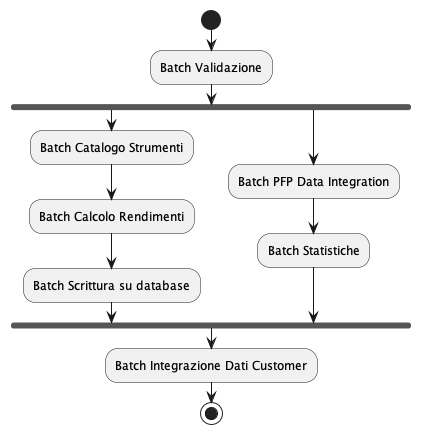
\includegraphics[width=.6\textwidth]{img/batch-dependency.png}
    \centering
    \caption{Rappresentazione grafica della \textit{step function} che esegue l'ETL del progetto.}
    \label{fig:batch-dependency}
\end{figure}

\subsection{Validazione}\label{subsec:etl-validation}
Il job di validazione si occupa di leggere tutti i flussi in input nel formato \textit{csv}, validarli, applicare delle trasformazioni e riscriverli in formato \textit{parquet}~\cite{parquet}.
Per poter validare i dati in input, è necessaria la configurazione di un tracciato che determini quale schema ci si aspetta dai flussi.
La validazione comprende diversi controlli per verificare quali record siano da scartare e quali possano passare alle fasi successive.
I controlli necessari sono:
\begin{itemize}
    \item Chiave primaria duplicata - la chiave primaria determina l'identificatore di un record;
    di conseguenza, i record con stessa chiave primaria sono da scartare in quanto non si sa quale sia corretto.
    \item Chiave esterna non censita - per i flussi che hanno una chiave esterna è necessario controllare che questa sia presente nel flusso di riferimento.
    Ad esempio, se esiste un rapporto su un determinato cliente, nel flusso relativo ai rapporti sarà presente la chiave del flusso dei clienti.
    Bisogna verificare se effettivamente esiste un cliente con quella chiave nell'apposito flusso, altrimenti il record del rapporto sarà da scartare.
    \item Campi obbligatori - nel tracciato deve essere indicato per ciascun campo se questo può essere \texttt{nullable} o meno.
    Di conseguenza, è necessario scartare tutti i record che presentano campi valorizzati a \texttt{null}, ma che sono considerati obbligatori.
    \item Tipi di dato - nel formato \textit{csv}, tutti i dati sono salvati come sequenza di caratteri;
    tuttavia, gli schemi successivi possono richiedere dei dati con tipi specifici, quali intero, booleano e altri.
    Diventa quindi necessario verificare che possa essere effettuato il \textit{cast} dei dati presenti nei flussi come indicato nel tracciato per ciascun campo.
\end{itemize}
Il caricamento in memoria dei flussi deve avvenire in modo efficiente per garantire le migliori prestazioni.
L'ordine con cui vengono caricati i flussi influisce sulle prestazioni e sul risultato della validazione in quanto questi controlli, assieme all'\textit{enrichment} dei dati, vengono fatti in sequenza sulle tabelle.
Ad esempio, per controllare il censimento di un record con chiave esterna, è necessario che il flusso con la \textit{foreign key} sia già stato importato.
Quindi, per ovviare a questo problema, si affronta una fase di caricamento che costruisce un ordine specifico sulla base del modello dei flussi.
Nello specifico si costruisce un \textbf{direct acyclic graph} (DAG) rappresentante le dipendenze dei flussi tra loro, dove una dipendenza può derivare da una chiave esterna o da altre necessità (come l'utilizzo di un flusso \textit{ad hoc} per arricchire i dati di un altro).
A partire dal DAG, si deduce la sequenza con cui vengono quindi ordinati i flussi;
questo rimane poi l'ordine con cui vengono mantenuti e con cui avvengono tutte i controlli e le trasformazioni.
La figura~\ref{fig:dag-model} mostra il DAG semplificato del modello trattato (non sono stati riportati tutti i campi in quanto non necessari per l'apprendimento di questa parte, così come non sono state riportate le chiavi primarie dei flussi per intero per rendere la figura più compatta).
\begin{figure}
    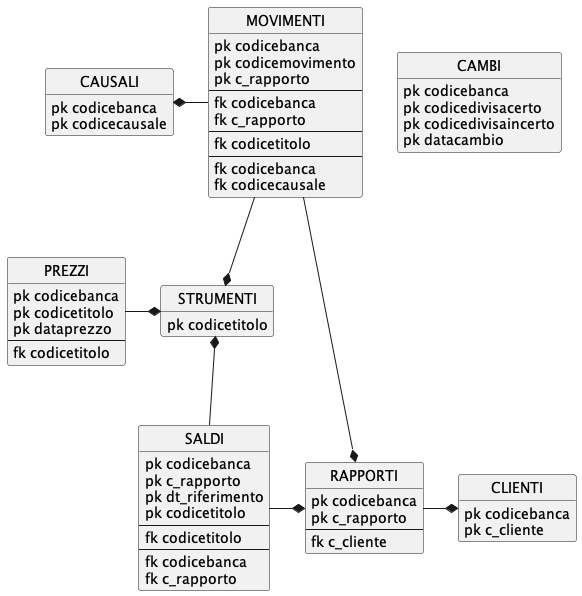
\includegraphics[width=\textwidth]{img/dag-model.png}
    \centering
    \caption{Grafo diretto aciclico delle dipendenza tra i flussi.}
    \label{fig:dag-model}
\end{figure}

Inoltre, i controlli producono due output: uno contenente i record validati, e l'altro quelli scartati.
Entrambi vengono salvati in formato \textit{parquet} all'interno di due repository sulla base della natura del flusso:
un flusso può essere ricevuto dal cliente \textit{in full} oppure \textit{in delta}, dove la prima opzione indica un flusso che viene mandato una volta sola poichè il suo contenuto non cambia, mentre la seconda indica flussi che continuano ad aumentare di volume e che vengono quindi inviati continuamente.
Per quanto riguarda i flussi \textit{in delta}, è stato pattuito col cliente che invii solo i nuovi record, in quanto non avrebbe senso processare informazioni che sono già state elaborate dall'\textit{ETL}.
Quindi, per distinguere le due tipologie di flusso, queste vengono salvate in due repository separate: \texttt{output/output} per i flussi \textit{in full} e \texttt{output/store} per quelli \textit{in delta}.
Invece, per distinguere flussi validi e non, gli scarti vengono salvati in un repository \texttt{output/output/errors} oppure \texttt{output/store/errors} a seconda del flusso;
inoltre, il cliente può accedere a questi repository, in modo tale da non dover comunicare errori nei flussi ogniqualvolta si verifichino, come da requisito (vedi sezione~\ref{subsec:problem-prometeia}).
Il concetto appena descritto è rappresentato nella figura~\ref{fig:full-delta}.
\begin{figure}
          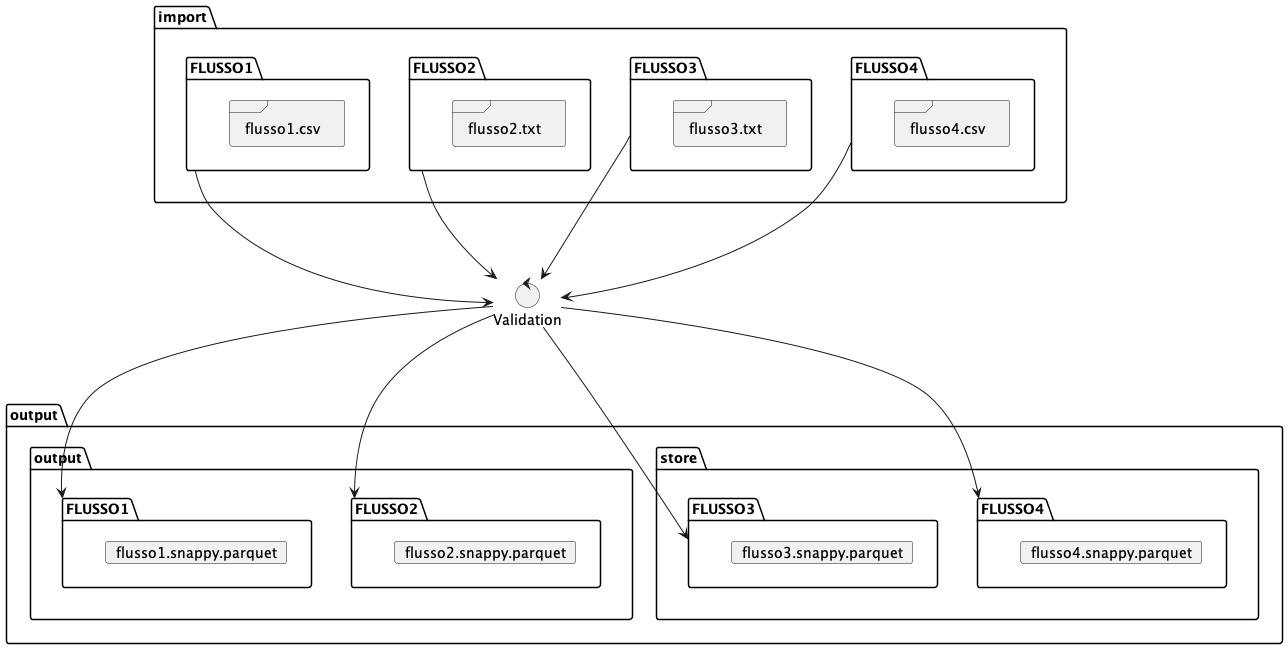
\includegraphics[width=\textwidth]{img/full-delta.png}
          \centering
          \caption{Processo di salvataggio dei file \textit{parquet}, distinguendo tra flussi \textit{in full} e \textit{in delta}.}
          \label{fig:full-delta}
\end{figure}

\subsection{Catalogo Strumenti}\label{subsec:etl-cat}
Il job di integrazione degli strumenti finanziari, soprannominato \textit{cat}, è necessario per mantenere integrato il contenuto del flusso riguardante i prodotti finanziari, uno dei flussi \textit{in full} più importanti.
Questo infatti contiene i riferimenti a tutti gli strumenti finanziari, ed è utilizzato da molteplici altri flussi per ottenere informazioni su di essi.
Quindi, affinchè quest'ultimo non contenga campi vuoti o campi superflui poiché non utilizzati, è necessario un job che si occupi appositamente della sua pulizia e integrazione.
In particolare, il job in questione prende in input i flussi in formato \textit{parquet} prodotti dal job di validazione e scrive su un indice \textbf{OpenSearch} in modo che diversi endpoint possano reperire queste informazioni tramite \textit{API REST}.

Questo batch ha il compito di integrare diverse informazioni presenti in flussi diversi all'interno di un unico indice.
In particolare, per ciascun strumento finanziario vanno reperite diverse informazioni presenti in flussi separati che contengono un riferimento al titolo dello strumento.
Quindi, la struttura di tale batch deve permettere di prendere in input solo determinati flussi, cioè quelli necessari ad integrare le informazioni sugli strumenti.
Una volta prelevate tali informazioni, può avvenire l'integrazione:
si può affermare che questa parte, se ben strutturata e priva di errori, non genererà errori dovuti ad incoerenze di schema come chiavi esterne non censite, dato che tali controlli sono già avvenuti nel batch della validazione descritto nella sezione~\ref{subsec:etl-validation}.
In seguito all'integrazione, gli strumenti finanziari saranno quindi completi e potranno essere generati i due principali output di questo batch:
\begin{itemize}
    \item Indicizzazione dei dati sugli strumenti e caricamento su \textit{OpenSearch}.
    \item Scrittura dei dati sugli strumenti in formato \textit{parquet} in una directory separata rispetto a quella del batch precedente.
\end{itemize}
La duplicazione dell'output è dovuta ai diversi casi d'uso di questi:
l'indice su \textit{OpenSearch} è storicamente utilizzato da diversi endpoint tramite \textit{API REST};
risultano quindi necessari la scrittura e l'aggiornamento di tale indice.
Invece, la scrittura delle medesime informazioni in \textit{cloud} in formato \textit{parquet} avviene per comodità:
infatti, potrebbe risultare scomodo per i batch successivi reintegrare determinate informazioni relative ad uno strumento finanziario quando tale operazione è già avvenuta.
Quindi, semplicemente si mantengono in directory separate il flusso ricavato dalla validazione e quello ottenuto dal catalogo.

\subsection{Calcolo Rendimenti}\label{subsec:etl-returns}
Il job dei rendimenti si occupa di calcolare i rendimenti per ciascun cliente su diverse finestre temporali (vedi sezione~\ref{subsec:problem-prometeia}).
Tale job prende in input i flussi in formato \textit{parquet} prodotti dalla validazione e li integra con i rendimenti calcolati sulla base delle finestre temporali richieste (che quindi costituiscono un parametro del job).
I risultati dei rendimenti, anche detti \textit{return items}, vengono ulteriormente scritti in formato \textit{parquet} in un repository \texttt{output/returnitems}.

\subsection{Scrittura su database}\label{subsec:etl-postgres}
Un requisito importante è costituito dalla scrittura dei \textit{return items} su un database \textit{PostgreSQL}.
Questa necessità è dovuta dall'esistenza di diverse componenti front end che reperiscono alcuni dati (non tutti) dei rendimenti direttamente da database \textit{Postgres}.
Di conseguenza, tale job si occupa di rileggere i rendimenti in formato \textit{parquet}, applicare alcune trasformazioni di pulizia e valorizzazione di campi aggiunti e scrivere il risultato su un database remoto.
Tali operazioni venivano precedentemente effettuate all'interno del job di calcolo dei rendimenti;
tuttavia, ci si è resi conto che la scrittura su database costituisce un collo di bottiglia piuttosto oneroso per quanto riguarda le prestazioni del job.
Di conseguenza, è stato deciso di dedicare un batch apposta per la scrittura, in modo tale da poterlo eseguire in parallelo alle fasi successive.

Per poter accedere al database, sono necessarie delle credenziali e una serie di informazioni utili per stabilire la connessione.
Queste informazioni costituiscono un \textit{asset} da proteggere in quanto concedono l'accesso a dati dei clienti:
risulta quindi necessario mantenerle all'interno di un segreto, cioè risorse protette sbloccabili solo tramite una chiave riservata.
Pertanto, è stato deciso di fare uso di \textit{AWS SecretsManager}.
Infatti, tale servizio deserializza le informazioni contenute all'interno del segreto che non potrebbero essere mantenute nei sorgenti del componente, come \textit{hostname} e \textit{password} del database.
Dopodiché procede con la scrittura di un sottoinsieme di informazioni sul database.

\subsection{Data Integration PFP}\label{subsec:etl-pfp}
L'integrazione dei dati del PFP è stata momentaneamente gestita in un batch separato da quello della validazione.
In futuro, con grande probabilità, questa componente verrà fusa con quella di validazione.
Questo batch ha lo scopo di reimplementare un modulo già presente e operativo in produzione, ma che necessita di una rivisitazione con nuove tecnologie per abbattere i lunghi tempi d'esecuzione.
A livello architetturale, presenta le stesse caratteristiche del batch di validazione.

\subsection{Statistiche}\label{subsec:etl-stats}
In preparazione per la fase finale, che prevede l'integrazione dei dati dei clienti finali della banca, è necessario reperire \textbf{massivamente} informazioni su di essi.
Le chiamate massive, sono così dette in quanto elaborano una serie di dati per ciascun cliente, richiedendo quindi un certo ammontare di tempo;
motivo per cui è stato ritenuto opportuno separarne l'esecuzione dai job precedenti e successivi.
Le informazioni in questione si ottengono chiamando degli \textit{engine} che effettuano calcoli sulla base dei dati presentati per ciascun cliente.
Affinchè queste informazioni possano essere reperite, è necessario calcolare delle statistiche su ciascun cliente che servono in input agli \textit{engine};
questo batch si occupa di calcolare tali statistiche e riscrivere tutti i flussi necessari nel formato richiesto dalle chiamate massive.

\subsection{Integrazione Dati \textit{Customer}}\label{subsec:etl-customer}
La fase finale consiste nel reperimento di tutte le informazioni ottenute durante le fasi precedenti, l'integrazione opportuna e la trasformazione in formato \textit{json} per poter scrivere il risultato su un indice \textbf{OpenSearch}.
Per poterlo fare, è necessaria la rilettura dei \textit{parquet} con i dati dei clienti e delle informazioni ottenute dalle chiamate massive.
Una volta raccolte tutte le informazioni necessarie per il risultato finale, sarà sufficiente individuare un modo per filtrare i dati da scrivere su indice e un modo per uniformare tutto in formato \textit{json}.

\section{Baseline}\label{sec:baseline-architecture}
Come anticipato nella sezione~\ref{sec:solution}, la parte del progetto Baseline realizzata durante il tirocinio è stata iniziata durante lo svolgimento dello stesso.
Lo scopo di questo progetto è quello di realizzare un prodotto che riesca ad emulare tutti gli step di un tipico progetto di ETL come quello discusso nella sezione~\ref{sec:etl-architecture}.
Le componenti da realizzare sono state individuate dagli analisti e dagli ingegneri di Prometeia osservando progetti con diverse caratteristiche in comune.
L'esigenza di partire con questo progetto per Baseline è nata per via della necessità di avere un catalogo interno degli strumenti finanziari.
Quindi, per la durata del tirocinio, l'avanzamento di questo progetto si è limitata al completamento del catalogo degli strumenti.
Eventuali componenti aggiuntive, come quella del calcolo dei rendimenti, verranno introdotte in momenti successivi.

Queste componenti hanno una dipendenza sequenziale (figura~\ref{fig:baseline-dependency}), in quanto la corretta esecuzione del secondo dipende fortemente dal successo del primo.
Alcuni casi d'uso del catalogo degli strumenti sono quello dell'analisi dati e quello del reperimento di informazioni sfruttando l'indice \textit{OpenSearch} come \textit{Software as a Service}.
\begin{figure}
    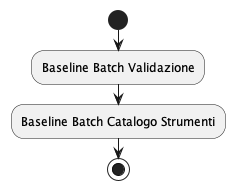
\includegraphics[width=.6\textwidth]{img/baseline-dependency.png}
    \centering
    \caption{Rappresentazione grafica della \textit{step function} che esegue i batch di Baseline.}
    \label{fig:baseline-dependency}
\end{figure}

\subsection{Validazione}\label{subsec:bl-validation}
Ha lo scopo di caricare i flussi necessari per ottenere tutte le informazioni del catalogo degli strumenti.
Nello specifico, si compone di due parti:
una prima parte che carica diversi flussi unicamente relativi agli strumenti in formato \textit{csv} e produce in output un flusso nel medesimo formato combinando le informazioni più adatte di ciascuno di quelli di input;
la seconda parte esegue la validazione di tutti i flussi necessari per integrare il catalogo degli strumenti, compreso quello prodotto dallo step precedente.
L'output della validazione corrisponde alla produzione di flussi in formato \textit{parquet}.

\subsection{Catalogo Strumenti}\label{subsec:bl-cat}
Questa fase ha lo scopo di leggere in input i file \textit{parquet} prodotti dallo step di validazione e integrare tutte le informazioni per ciascuno strumento finanziario.
Idealmente, ogni flusso validato contiene una chiave con il codice del titolo, che rappresenta la chiave degli strumenti.
Quindi, un compito importante di questo \textit{job} è quello di raggruppare ciascun record per il codice del titolo ed effettuare un'operazione di \textit{join} per ogni strumento con tutti i flussi necessari.
Una volta integrate tutte le informazioni, il risultato ottenuto viene scritto su un indice \textit{OpenSearch}.

\section{Infrastruttura}\label{sec:infrastructure}

Come anticipato, Prometeia utilizza le tecnologie di \textit{Amazon Web Services} per avere supporto in \textit{cloud}.
Il \textit{cloud service provider} di Amazon mette a disposizione una serie di servizi che possono essere sfruttati per diversi scopi, tra cui hosting e storing.
Questo capitolo riassume l'architettura utilizzata per mantenere le risorse in \textit{cloud} e permettere la loro interazione.

\subsection{Hosting}\label{subsec:hosting}
I progetti sviluppati sono stati mantenuti in dei repository \textit{GitHub}.
In particolare, Prometeia ha diverse organizzazioni sul sito citato;
generalmente, una per ciascuna area di competenza.
Il tirocinio si è svolto all'interno dell'area di \textbf{WAM} (\textit{Wealth and Asset Management}), che coinvolge diversi team e riguarda lo sviluppo di sistemi per il benessere dei clienti delle banche.
Ne consegue che l'organizzazione \textit{GitHub} che ha mantenuto i repository dei progetti è stata \textit{prometeia-wam}.
All'interno di tale organizzazione sono stati creati diversi repository, diversificati per cliente e tecnologie utilizzate.
Ad esempio, relativamente al progetto di questa tesi, sono stati creati, per i diversi progetti, i repository
\begin{itemize}
    \item \texttt{<progetto>-scala-spark},
    \item \texttt{<progetto>-product-catalog},
\end{itemize}
dove il primo contiene codice \textit{Scala} che sfrutta la tecnologia \textit{Spark} per realizzare l'architettura descritta nela sezione~\ref{sec:etl-architecture}, mentre il secondo contiene esclusivamente il sorgente del batch \textit{Catalogo Strumenti}.
La diversificazione è stata fatta in quanto il secondo progetto è stato realizzato utilizzando \textit{Python} per questioni di flessibilità del codice, poiché tale batch necessita di scrivere su un indice \textit{OpenSearch}.
La scelta del linguaggio \textit{Python} per tale componente è stata fatta per via dell'esistenza di una libreria che facilita la scrittura su indice: \texttt{opensearchpy}.
I nomi dei repository sono stati rispettivamente \texttt{baseline-scala-spark} e \texttt{baseline-product-catalog} per quanto riguarda il progetto Baseline.
Per il progetto esterno, realizzato per il cliente, è stato semplicemente inserito il nome dello stesso.

Tornando al primo repository, esso contiene la maggior parte del lavoro svolto.
Ogni batch descritto nela sezione~\ref{sec:etl-architecture} è stato sviluppato all'interno del repository in questione, come programma \textit{Scala}.
In particolare, ogni batch viene inizializzato a partire da un \textit{main} apposito che richiama risorse interne al progetto oppure di prodotto, quindi librerie esterne, ma comunque sviluppate internamente a Prometeia.
Per dare un'idea più chiara della struttura interna al repository, la figura~\ref{fig:packages-structure} mostra il contenuto del repository, senza andare nel dettaglio di ciascun package.
\begin{figure}
    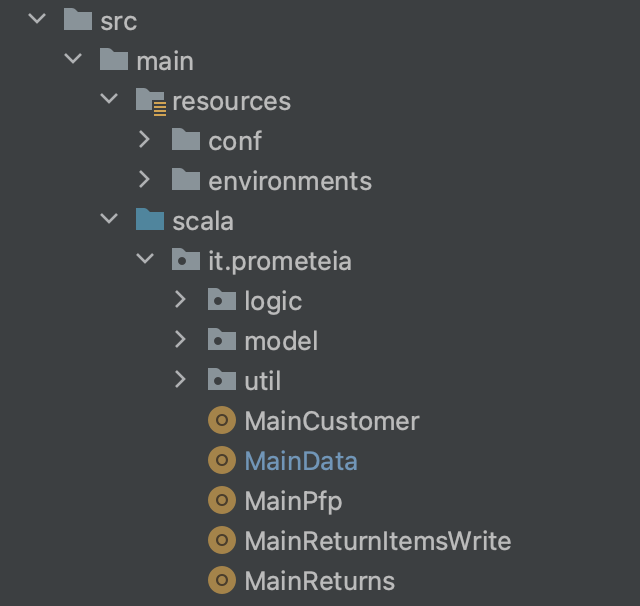
\includegraphics[width=.6\textwidth]{img/packages-structure.png}
    \centering
    \caption{Programmi \textit{main} del progetto \textit{Scala} e i package contenuti nel repository di sviluppo.}
    \label{fig:packages-structure}
\end{figure}
Un altro dei vantaggi offerti da \textit{GitHub} è quello delle \textbf{GitHub Actions}.
Infatti, queste permettono di realizzare delle \textit{pipeline} di \textit{continuous integration} internamente ai repository.
Tale servizio è stato sfruttato per eseguire il \textit{deploy} di una versione funzionante dei programmi realizzati.

\subsection{Deployment}\label{subsec:deployment}
Il \textit{deployment} dei sistemi viene gestito in un contesto \textbf{multi-environment}, in cui ogni ambiente ha obiettivi precisi.
Nello specifico, Prometeia ha individuato un insieme di ambienti sui quali operano diverse entità con diverse funzionalità:
\begin{itemize}
    \item \textbf{Sviluppo} - Soprannominato \textit{dev}, consiste nell'ambiente su cui vengono create e testate le applicazioni.
    Gli sviluppatori, seguendo determinati standard, costruiscono i sistemi in questo ambiente testandoli da diversi punti di vista.
    Questo ambiente non è visibile ai clienti, per cui eventuali errori sono accettabili.
    Non per niente, è l'ambiente in cui si verificano errori con maggiore frequenza;
    infatti, in fase di sviluppo le soluzioni non sono ancora sufficientemente stabili e necessitano di ulteriori test per individuare bug.
    \item \textbf{Staging} - Soprannominato \textit{stag}, è l'ambiente in cui vengono trasferite le feature che si vogliono presentare al cliente tramite \textit{demo}.
    Consiste nell'ambiente su cui gli analisti effettuano la maggior parte delle verifiche per individuare eventuali \textit{bug} o errori da risolvere.
    L'incorrere di errori in questo ambiente è generalmente allarmante poiché significa aver tralasciato aspetti importanti in ambiente di sviluppo.
    \item \textbf{Pre-produzione} - Soprannominato \textit{preprod}, è un ambiente condiviso con il cliente che quindi può impiegare analisti per ulteriori verifiche.
    Consiste in un'area in cui il cliente può effettivamente analizzare il lavoro svolto per verificare che coincida con i requisiti e le aspettative.
    \item \textbf{Produzione} - Soprannominato \textit{prod}, è l'ambiente su cui viene effettuato il \textit{deployment} delle applicazioni finali, le quali diventano quindi disponibili e utilizzabili dagli utenti.
    Gli errori in produzione sono inaccettabili, motivo per cui, quando si carica qualcosa su questo ambiente, bisogna agire con attenzione e cautela.
    \item \textbf{Ambiente Bolla} - Un ambiente aggiuntivo considerato una copia della produzione su cui effettuare dei test.
    Nello specifico, consiste in una replica dello stato dell'ambiente di produzione impiantato ad una determinata data.
    In questo modo, è possibile testare nuovi sviluppi prima di renderli effettivi in produzione con le stesse condizioni, verificando che non avverranno errori al momento dell'\textit{upgrade}.
\end{itemize}
Ad esclusione di \textit{dev}, tutti gli altri ambienti vengono definiti \textbf{multitenant}.
Infatti, i permessi di accesso a questi ambienti si dividono in due macrogruppi:
\begin{itemize}
    \item \texttt{permessi-dev}, che permettono di accedere all'ambiente di sviluppo e sono concessi a tutte le risorse coinvolte nello sviluppo dei progetti;
    \item \texttt{permessi-mt}, che permettono di accedere a tutti gli ambienti oltre a quello di sviluppo;
    questi sono concessi solamente a risorse con alta responsabilità all'interno dei progetti.
\end{itemize}

Il \textit{deployment} è gestito in modo automatico solamente in ambiente di sviluppo.
In particolare, è stato scelto di caricare la versione aggiornata dei progetti solamente nel caso di \textit{push} sul branch \textit{develop}.
Infatti, ogni progetto mantenuto su \textit{GitHub} è dotato di un \textit{workflow} che viene eseguito nei casi citati, simile a quello mostrato nel listato~\ref{code:deploy}.
Nello specifico, questi flussi di \textit{continuous integration} eseguono:
\begin{enumerate}
    \item una \textit{build} del repository con \textbf{Maven} come strumento di \textit{build automation},
    \item l'autenticazione con credenziali di \textit{Amazon Web Services},
    \item la copia della libreria prodotta e dei \textit{main} su un bucket di S3.
\end{enumerate}
In questo modo, eseguendo la pipeline, è possibile ottenere il \textit{deploy} di una versione funzionante dei programmi realizzati.
Una volta effettuato il \textit{deploy} dei programmi, è possibile lanciarli manualmente e individualmente dal servizio \textit{Glue}:
quando l'intero sistema verrà rilasciato in produzione, questo verrà eseguito in sequenza con una determinata frequenza, ad esempio una volta al giorno;
per ora, vengono eseguiti manualmente i singoli batch per produrre flussi in output e testare il risultato prodotto (il testing del sistema viene discusso nella sezione~\ref{subsec:testing}).

\subsection{Testing}\label{subsec:testing}
La creazione di suite di test per i sistemi di ETL realizzati in Spark risulta essere problematica.
Innanzitutto, la realizzazione di \textit{Unit Test} per ogni trasformazione sarebbe complessa:
per via della natura dichiarativa delle trasformazioni di Spark (discussa nella sezione~\ref{subsec:datasets}), testare i \textit{Dataset} risultanti consisterebbe nella semplice verifica delle dimensioni di questi, in termini di record, ma anche di campi o colonne.
Inoltre, alcune feature non sarebbero testabili in quanto presenterebbero comportamenti diversi in locale o su un cluster.
Diverse procedure in Spark presentano caratteristiche diverse a seconda di quanti nodi vengono utilizzati per il calcolo distribuito.
Un esempio è la funzione colonna \texttt{monotonically\_increasing\_id}:
quest'ultima genera numeri interi a 64 bit \textit{monotonically increasing}, cioè crescenti, ma non necessariamente consecutivi.
Quindi tale funzione riesce ad assegnare un numero unico e identificativo ad ogni record, ma la sua implementazione potrebbe essere male interpretata.
Infatti, per ogni id, essa inserisce il numero identificatore della partizione corrente nei primi 31 bit, e il numero del record all'interno della partizione nei restanti 33 bit.
Per esempio, supponendo di avere un \textit{Dataset} con 2 partizioni, ognuna contente 3 record, la funzione \texttt{monotonically\_increasing\_id} restituirebbe i seguenti id:
\[0, 1, 2, 8589934592, 8589934593, 8589934594.\]
Si puo notare come tutti i numeri siano effettivamente unici.
Tuttavia, non rappresentano il numero effettivo della riga all'interno dell'intero \textit{Dataset}.
Di fatto, ciò è valido solo per i primi 3 id, cioè quelli corrispondenti alla prima partizione.
Questo perchè il numero della prima partizione corrisponde intuitivamente a 0, quindi l'id risultante corrisponde a quello del numero record inserito negli ultimi 33 bit.
Come si può capire, questa funzione presenta comportamenti diversi a seconda del numero di nodi disponibili per un determinato \textit{job};
di conseguenza, l'individuazione di \textit{Unit Test} adatti per un \textit{Dataset} che la utilizza risulterebbe difficile.

Per come è stata pensata l'infrastruttura dei sistemi, il momento adatto per eseguire delle ipotetiche suite di test sarebbe quello precedente al \textit{deployment} con le \textit{GitHub Actions}.
Tuttavia, per i motivi sopra citati non sono stati inseriti controlli con test nella procedura di \textit{deployment}.
Quindi, per testare i sistemi realizzati sono stati utilizzati principalmente due metodi:
\begin{itemize}
    \item Esecuzione dei batch in locale con un sottoinsieme di dati estremamente ridotto.
    \item Analisi dati tramite query sul servizio \textit{AWS Athena} in seguito all'esecuzione dei job su \textit{AWS Glue}.
\end{itemize}
A seconda delle problematiche da risolvere o delle feature da introdurre, sono stati utilizzati l'uno o l'altro approccio o entrambi.

Per quanto riguarda il primo approccio, è stato preso un sottoinsieme di record per ciascun flusso, facendo particolare attenzione che i record scelti restituiscano delle \textit{join} non vuote.
Quindi, per testare delle feature che coinvolgono l'operazione di \textit{join} o altre trasformazioni, sono stati testati i sistemi eseguendoli in modalità di \textit{debug}, e verificando che il risultato effettivo corrisponda a quello atteso, oltre che non si presentino errori a \textit{runtime}.
La riduzione dei flussi è stata fatta in quanto eseguire i batch in locale con i dati completi richiederebbe diverse ore per ciascun batch;
mentre l'esecuzione effettiva sui cluster di AWS richiede pochi minuti.

Per quanto riguarda il secondo approccio, viene generalmente utilizzato dagli analisti per confermare la correttezza delle feature introdotte, ma viene anche utilizzato dagli sviluppatori per verificare casi specifici e delicati come quello della \texttt{monotonically\_increasing\_id} descritto sopra.
In alcuni casi, l'esecuzione in locale dei batch non risulta sufficiente per verificare l'esattezza di una feature.
Ad esempio, volendo testare dei comportamenti particolari dovuti alla natura distribuita di Spark oppure casi specifici come informazioni relative a uno strumento finanziario in particolare.
Per questi casi quindi la prassi è quella di effettuare delle query su \textit{AWS Athena} in seguito all'esecuzione dei job su \textit{Glue}.
Spesso, tali query vengono fornite a priori dagli analisti, i quali conoscono bene il risultato atteso e perciò sono anche qualificati per l'individuazione di queste.

\subsubsection{Crawlers}\label{subsubsec:crawlers}

Per comprendere il modo in cui vengono effettuati i test, è necessario citare il servizio \textit{Crawlers} di AWS Glue.
Tale servizio è in grado di sopperire alla problematica della lettura dei file in formato \textit{parquet}:
in particolare, come è stato anticipato nella sezione~\ref{subsec:etl-validation}, in seguito alla validazione i flussi vengono riscritti nel formato citato per garantire delle migliori prestazioni in lettura per i processi successivi.
Tuttavia, la scelta di salvataggio dei dati in file di formato binario ne complica il testing.
La scelta migliore per poter effettuare agilmente delle query su di essi sarebbe quella di mantenerli all'interno di un database relazionale:
infatti, all'interno dei database relazionali, la strutturazione dei contenuti è rigida;
i dati vengono normalizzati e inseriti in delle tabelle, quindi salvati secondo un preciso schema.
Lo schema definisce righe, colonne, indici, relazioni tra tabelle e ulteriori elementi e attua l’integrità referenziale nelle relazioni~\cite{rdbms-vantaggi}.
Invece, nei file in formato \textit{parquet}, così come in altri formati o altre tecnologie, i dati vengono salvati senza tabelle né schemi univoci.
Nel caso corrente, la dipendenza dall'infrastruttura in \textit{cloud} è stata prevalente rispetto alla comodità della strutturazione rigida dei database relazionali, quindi è stato adoperato il servizio dei \textit{crawlers} di AWS Glue per risolvere tale problema.
I \textit{crawler} sono processi eseguibili che permettono di creare definizioni di tabelle a partire da file non strutturati.
Di fatto, costituiscono il collegamento tra il \textit{datastore} rappresentato dai bucket di S3 e il \textit{query editor} di Amazon Athena.
Possono essere configurati con dei parametri come il percorso dei file da analizzare e il loro formato.
Quando eseguiti, questi vanno a leggere tutti i file nel formato e percorso specificati ed effettuano un'analisi che permette di dedurre lo schema relazionale tra di essi.
A partire dallo schema, vengono creati dei metadati che puntano ai file \textit{parquet}.
In questo modo, Amazon Athena punta direttamente a questi metadati, garantendo la possibilità di effettuare analisi con delle query in linguaggio SQL.
Quindi, i \textit{crawler} vengono rieseguiti ogniqualvolta vi sia un cambiamento nello schema dei flussi.

Nel caso del progetto in questione, sono stati creati diversi \textit{crawler} a seconda del diverso percorso dei file mantenuti sullo storage di S3:
\begin{itemize}
    \item \texttt{input-crawler} - tale \textit{crawler} permette di inferire lo schema relazionale di file in formato \textit{csv} in input.
    Di fatto, la possibilità di effettuare query anche sui flussi ricevuti in input permette di confermare la correttezza di questi e di effettuare confronti per verificare la presenza di record prima e dopo l'esecuzione dei batch.
    \item \texttt{output-crawler} - tale \textit{crawler} esamina i file in formato \textit{parquet} esclusivamente di flussi \textit{in full} poiché separati da quelli \textit{in delta}.
    \item \texttt{scarti-crawler} - tale \textit{crawler} analizza i record scartati.
    È utile per controllare il motivo degli scarti;
    infatti, quando un record viene scartato dalla validazione, al suo \textit{DataFrame} viene aggiunta una colonna denominata \texttt{motivo\_scarto} che ne contiene la causa.
    \item \texttt{store-crawler} - tale \textit{crawler} analizza i record dei file storicizzati, cioè appartenenti a flussi \textit{in delta}.
    \item \texttt{returns-crawler} - tale \textit{crawler} esamina i file in formato \textit{parquet} salvati dopo l'esecuzione del batch dei rendimenti.
\end{itemize}

\section{Sviluppi futuri}\label{sec:future}

In questa sezione si elencano i possibili sviluppi futuri dell'architettura e dell'infrastruttura, ideati durante il tirocinio a fronte delle possibilità offerte dalle tecnologie utilizzate.

\subsection{Omogeneità di linguaggi}\label{subsec:future-cat}
Uno sviluppo futuro programmato è quello di rimuovere completamente le dipendenze dalla libreria \texttt{opensearchpy} in modo da non avere componenti realizzate in Python.
Come già anticipato, le componenti realizzate in Python tendono a rallentare le prestazioni:
siccome Spark è realizzato in Scala, quando vengono utilizzate le API di Python la libreria deve necessariamente trasformare gli oggetti da un linguaggio all'altro.
Questa trasformazione riduce esponenzialmente le prestazioni dei \textit{job} allo scalare della quantità di dati in input.
Di conseguenza, si considera opportuno rimuovere le dipendenze dalla libreria citata e migrare le componenti realizzate in Python al linguaggio Scala.
La soluzione ideale sarebbe quella di realizzare a prodotto una logica che permetta di definire il \textit{mapping} diretto a partire dal modello delle tabelle in Spark a quello degli indici di OpenSearch.
Una prima idea da cui si potrebbe impostare tale logica è descritta nella sezione~\ref{subsubsec:customer}.

\subsection{Passaggi di feature a prodotto}\label{subsec:future-customer}
Mano a mano che vengono realizzati componenti di ETL per diversi progetti, ci si rende conto che alcune feature risultano essere estremamente simili.
In particolare, l'obiettivo è quello di non duplicare logiche e ottenere uno standard riapplicabile nel momento in cui entrano in gioco dei nuovi progetti.
In questo modo, sarà possibile avere un'unica implementazione, corretta e testata, di feature somiglianti tra loro.
Come descritto nella sezione~\ref{sec:solutions}, è possibile realizzare soluzioni a prodotto rendendole estendibili (ad esempio, con una libreria), oppure mantenendole all'interno di servizi a sè stanti.
Nel caso del progetto in questione, è già successo che si trasferissero logiche all'interno della libreria di base che implementa l'ETL, e si continuerà a procedere in tale maniera.
Questa procedura, non deve avvenire solo quando si notano somiglianze con progetti già realizzati, ma deve anticipare il più possibile casi d'utilizzo futuri;
nel senso che nel momento in cui si realizzano soluzioni sapendo di poterle riutilizzare in futuro, queste dovrebbero essere implementate "a prodotto" piuttosto che "a progetto".

Un esempio di feature realizzata immediatamente "a prodotto" è quella del reperimento di segreti da \textit{AWS SecretsManager}, descritta nella sezione~\ref{subsec:etl-postgres}.
Infatti, sono diversi i progetti che necessitano di comunicare con entità esterne, e mantenerne le informazioni di accesso all'interno del codice sorgente rappresenta un rischio elevato di \textit{disclosure}.
Di conseguenza, è stato ritenuto opportuno sin da subito parametrizzare la logica di reperimento del segreto dal servizio di \textit{Amazon Web Services} e inserirla in libreria, in modo tale da poterla riutilizzare ed estendere in progetti futuri.

\subsection{Console per l'aggiornamento di flussi}\label{subsec:future-console}
Uno degli svantaggi dell'architettura individuata è rappresentato dal caso in cui i clienti sbaglino a inviare flussi;
in particolare, in casi in cui il flusso non è corretto per una porzione minima, come un singolo campo in un singolo record.
La procedura seguita al momento per questi casi consiste nel notificare il cliente dell'avvenuto e attendere il flusso corretto, oppure applicare la modifica manualmente;
tuttavia, la seconda opzione non andrebbe seguita in quanto, una volta accordato il tracciato dei flussi, è compito del cliente rispettarlo e assicurarsi della correttezza dei record inviati.
Comunque, tale procedimento può causare dei lunghi tempi di attesa che rallentano e possono bloccare gli sviluppi del progetto;
non solo quando si stanno testando feature in ambiente di sviluppo, ma soprattutto quando ne si effettua l'\textit{upgrade} in ambienti \textit{multitenant}.
Quindi, la situazione ideale coincide con la possibilità per il cliente di applicare modifiche direttamente sui flussi validati o sui flussi caricati in input sui bucket di \textit{AWS S3}.
Questa soluzione si potrebbe raggiungere con la realizzazione di una console \textit{ad hoc} accessibile dal cliente che permetta di visualizzare ed effettuare modifiche ai flussi nelle varie fasi dell'ETL.
Tuttavia, per quanto la lettura dei file dai bucket sia relativamente facile, non si può dire lo stesso della loro modifica:
infatti, nemmeno le funzionalità di \textit{Athena} consentono di effettuare operazioni di \textit{update} sui file.
Però esiste una possibile integrazione con le tabelle in formato \textit{Apache Iceberg} che permette di effettuare operazioni come l'inserimento o l'aggiornamento di record.
Inoltre, il design della specifica Iceberg è ottimizzato per il suo utilizzo su Amazon S3, garantendo anche la correttezza dei dati in scenari di scrittura simultanea~\cite{apache-iceberg}.
Riuscendo a realizzare una API per l'aggiornamento di tabelle direttamente sui file di S3, sarebbe possibile utilizzarla in una console in cui il cliente potrebbe effettuare query \textit{on the fly}, eliminando completamente i tempi d'attesa dei casi sopra citati.
